\documentclass[11pt,a4paper,reqno]{amsart}

\newcommand{\AppSection}[2]{%
    \clearpage
    \section*{#1}\label{#2}
}

\newcommand{\AppSubsection}[1]{%
    \clearpage
    \Needspace{8\baselineskip}
    \subsection*{#1}
}

\newcommand{\StrictFigure}[4]{%
    \par\medskip
    \begin{center}
        \includegraphics[#1]{#2}
        \captionof{figure}{#3}
        \label{#4}
    \end{center}
    \par\medskip
}

\newcommand{\StrictFigurePair}[8]{%
    \par\medskip
    \noindent
    \begin{minipage}[t]{0.48\linewidth}
        \centering
        \includegraphics[#1]{#2}
        \captionof{figure}{#3}
        \label{#4}
    \end{minipage}
    \hfill
    \begin{minipage}[t]{0.48\linewidth}
        \centering
        \includegraphics[#5]{#6}
        \captionof{figure}{#7}
        \label{#8}
    \end{minipage}
    \par\medskip
}

\usepackage{capt-of}
\usepackage{needspace}
% --- Packages ---
\usepackage[utf8]{inputenc}
\usepackage[T1]{fontenc}
\usepackage{amsmath,amsfonts,amssymb,amsthm}
\usepackage{mathtools}
\usepackage{mathpazo}
\usepackage{microtype}
\usepackage{booktabs}
\usepackage{array}
\usepackage{graphicx}
\usepackage{enumitem}
\usepackage{etoolbox}
\usepackage{placeins}
\usepackage{float}

% --- Layout & Geometry ---
\usepackage[margin=1.1in, footskip=0.4in]{geometry}
\renewcommand{\baselinestretch}{1.05}
\emergencystretch=2em

% --- Colors & Hyperlinks ---
\usepackage[dvipsnames]{xcolor}
\definecolor{DarkNavy}{RGB}{20, 40, 80}
\usepackage[
    colorlinks=true,
    linkcolor=DarkNavy,
    citecolor=DarkNavy,
    urlcolor=DarkNavy,
    bookmarksnumbered=true
]{hyperref}
\urlstyle{same}

% --- Theorem Environments ---
\newtheorem{theorem}{Theorem}[section]
\newtheorem{lemma}[theorem]{Lemma}
\newtheorem{proposition}[theorem]{Proposition}
\newtheorem{corollary}[theorem]{Corollary}

\theoremstyle{definition}
\newtheorem{definition}[theorem]{Definition}
\newtheorem{example}[theorem]{Example}
\newtheorem{assumption}[theorem]{Assumption}

\theoremstyle{remark}
\newtheorem{remark}[theorem]{Remark}

\numberwithin{equation}{section}

% --- Custom Math Macros ---
\newcommand{\R}{\mathbb{R}}
\newcommand{\N}{\mathbb{N}}
\newcommand{\E}{\mathbb{E}}
\newcommand{\dx}{\,\mathrm{d}x}
\newcommand{\grad}{\nabla}
\newcommand{\divg}{\nabla \cdot}
\newcommand{\norm}[1]{\left\lVert #1 \right\rVert}
\newcommand{\abs}[1]{\left\lvert #1 \right\rvert}
\newcommand{\tr}{\operatorname{tr}}
\newcommand{\diag}{\operatorname{diag}}
\newcommand{\softmax}{\operatorname{softmax}}
\newcommand{\relu}{\operatorname{ReLU}}
\newcommand{\vM}{\operatorname{vM}}
\newcommand{\concat}{\operatorname{Concat}}
\newcommand{\MLP}{\operatorname{MLP}}
\newcommand{\LayerNorm}{\operatorname{LayerNorm}}
\newcommand{\PhysicsAttn}{\operatorname{PhysicsAttn}}
\newcommand{\FeedForward}{\operatorname{FeedForward}}
\newcommand{\rank}{\operatorname{rank}}
\newcommand{\Integrator}{\operatorname{Integrator}}
\newcommand{\Vectorize}{\operatorname{Vectorize}}
\newcommand{\Scalarize}{\operatorname{Scalarize}}
\newcommand{\EquiFrame}{\operatorname{EquiFrame}}

% --- Metadata ---
% --- Metadata ---
\title[Inductive Biases and Learning Strategies for Learning Dynamics of Continuous Matter]{%
Inductive Biases and Learning Strategies for Learning Dynamics of Continuous Matter%
}

\author[JACOPO SENONER]{%
Jacopo Senoner\\
{\scriptsize EPFL, Lausanne, Switzerland}\\
{\scriptsize \texttt{jacopo.senoner@epfl.ch}}%
}

\makeatletter
% Title-page author: stop amsart from uppercasing \authors
\patchcmd{\@setauthors}
  {\MakeUppercase{\authors}}
  {\authors}
  {}
  {\typeout{Failed to patch title-page author capitalization}}

% Running header author: stop amsart from uppercasing \shortauthors
\patchcmd{\maketitle}
  {\@nx\MakeUppercase{\the\toks@}}
  {\the\toks@}
  {}
  {\typeout{Failed to patch running-header author capitalization}}
\makeatother

\date{}

\address{EPFL, Lausanne, Switzerland}
\email{jacopo.senoner@epfl.ch}

% ---------------------------------------------------------
\begin{document}

\begin{abstract}
We study how architectural and training inductive biases affect learned simulators for continuous matter, using the deformation dynamics of a three-dimensional damped cantilever beam as benchmark. The learning problem is formulated in the Graph Network-based Simulator framework: a neural model predicts the next-step acceleration and stress from a short history of mesh states, and an integrator rolls the prediction forward autoregressively. We compare a local message-passing baseline, MeshGraphNet, against equivariant local frames (ClofNet), local attention (GATv2), hierarchical pooling (Graph U-Net), and global attention through physical tokens (Transolver). We also study graph-connectivity augmentation, stress-target choices, noise-based rollout robustness, and physics-motivated residuals. The main empirical conclusion is that globality is useful: connectivity augmentation is effective but depends on how it's implemented, and Transolver's global attention gives the best overall performance across stress and rollout metrics. Online noising is the most important training bias for mitigating exposure bias, full-stress supervision outperforms von Mises-only supervision, and simple residual penalties are helpful mainly as secondary regularizers rather than game-changing constraints.
\end{abstract}

\maketitle

\subsection*{Acknowledgments}

This work was carried out under the supervision of Kevin Steiner, at IMOS Lab, EPFL. 

\section{Introduction}
\label{sec:intro}

Learning the dynamics of continuous matter is a central problem in scientific machine learning and computational mechanics. Classical finite element methods solve partial differential equations on meshes, but each new rollout can be expensive when one needs many trajectories, optimization loops, etc. Neural simulators aim to amortize this cost by learning a surrogate neural network from data. In this project the surrogate is trained on trajectories generated by a finite element simulation of a damped three-dimensional beam and evaluated by autoregressive rollout.

The particular beam task is intentionally demanding, as explained in Section~\ref{sec:problem-model}. The project therefore asks not only whether a neural simulator can fit the data, but which inductive biases are useful for this class of dynamics. Moreover, for each solution, whether successful or unsuccessful, we aim to briefly explain why it works or fails.

The report is organized as follows. Section~\ref{sec:problem-model} introduces the mechanics model, discretization, targets, dataset, and evaluation quantities. Section~\ref{sec:methodology} defines the learning framework and compares the architectural families studied in the project. Section~\ref{sec:results} presents the main experimental results. Section~\ref{sec:ablations} analyzes the most important ablations: connectivity/globality, noise, residuals, target choices, features, and implementation choices. Section~\ref{sec:conclusions} summarizes the main takeaways and Section~\ref{sec:futurework} explains future directions.

The guiding research questions are the following.
\begin{enumerate}[label=\textbf{RQ\arabic*.}, leftmargin=2.2cm]
    \item Which architectural biases are best suited to the deformation dynamics of a damped 3D beam: local message passing, equivariance, hierarchical pooling, local attention, or global attention?
    \item Is global information best introduced at the architecture level, for example through Transformers, or at the graph-connectivity level, for example through $k$-hop, wall, or random edge augmentation in MPNN networks?
    \item Which training biases improve autoregressive robustness and physical fidelity: online noise, target correction, stress-target design, or physics-motivated residual losses?
\end{enumerate}

\section{Problem Model}\label{sec:problem-model}

\subsection{Physical model}

The physical system is a cantilever beam occupying the rectangular domain
\begin{equation}
    \Omega = [0,L]\times [0,W]\times [0,D] \subset \R^3.
\end{equation}
The beam is clamped on one side and driven by a traction ramp on the opposite boundary. Let $u:\Omega\times[0,T]\to\R^3$ denote displacement. For Young's modulus $E$, Poisson ratio $\nu$, density $\rho$, mass damping coefficient $\eta_m$, and stiffness damping coefficient $\eta_k$, define the Lam\'e parameters and infinitesimal strain by
\begin{equation}
    \mu = \frac{E}{2(1+\nu)},
    \qquad
    \lambda = \frac{E\nu}{(1+\nu)(1-2\nu)},
    \qquad
    \varepsilon(u)=\frac{1}{2}\left(\grad u + \grad u^\top\right).
\end{equation}
The Cauchy stress for linear isotropic elasticity is
\begin{equation}
    \sigma(u)=2\mu\varepsilon(u)+\lambda\tr(\varepsilon(u))I.
\end{equation}
The damped beam equation used to generate the data is
\begin{equation}
\left\{
\begin{aligned}
    \rho \ddot u + \eta_m \rho \dot u - \divg\left(\sigma(u)+\eta_k\sigma(\dot u)\right) &= f && \text{in } \Omega\times(0,T),\\
    \sigma(u) &= 2\mu\varepsilon(u)+\lambda\tr(\varepsilon(u))I && \text{in } \Omega\times(0,T),\\
    u &= \bar u && \text{on } \Gamma_D\times(0,T),\\
    \left(\sigma(u)+\eta_k\sigma(\dot u)\right)n &= \bar t && \text{on } \Gamma_N\times(0,T),\\
    u(x,0)&=u_0(x),\qquad \dot u(x,0)=v_0(x) && \text{in } \Omega.
\end{aligned}
\right.
\label{eq:pde}
\end{equation}
The finite element solver uses continuous piecewise-linear displacement fields, i.e. CG1 displacement. Stress is first computed in a discontinuous piecewise-constant tensor space, i.e. DG0, and is then projected or evaluated as nodewise CG1 targets for the graph-learning problem.

In the final dataset, the material parameters are constant and are not given explicitly as inputs to the neural network:
\begin{equation}
    E=1000,\qquad \nu=0.3,
    \qquad \rho=1,
    \qquad \eta_m=\eta_k=0.01.
\end{equation}
Thus the model is not learning how material parameters vary across materials; rather, it learns the fixed material response implicitly from trajectories.

Overall, the task contains several challenging behaviours: the predicted dynamical target is second order in time, since the model predicts acceleration; the motion is non-quasi-static and ``wobbly'' ($\approx$ high-frequency); the system is three-dimensional; and the response combines local elastic interactions with global deformation modes.

\begin{figure}[H]
    \centering
    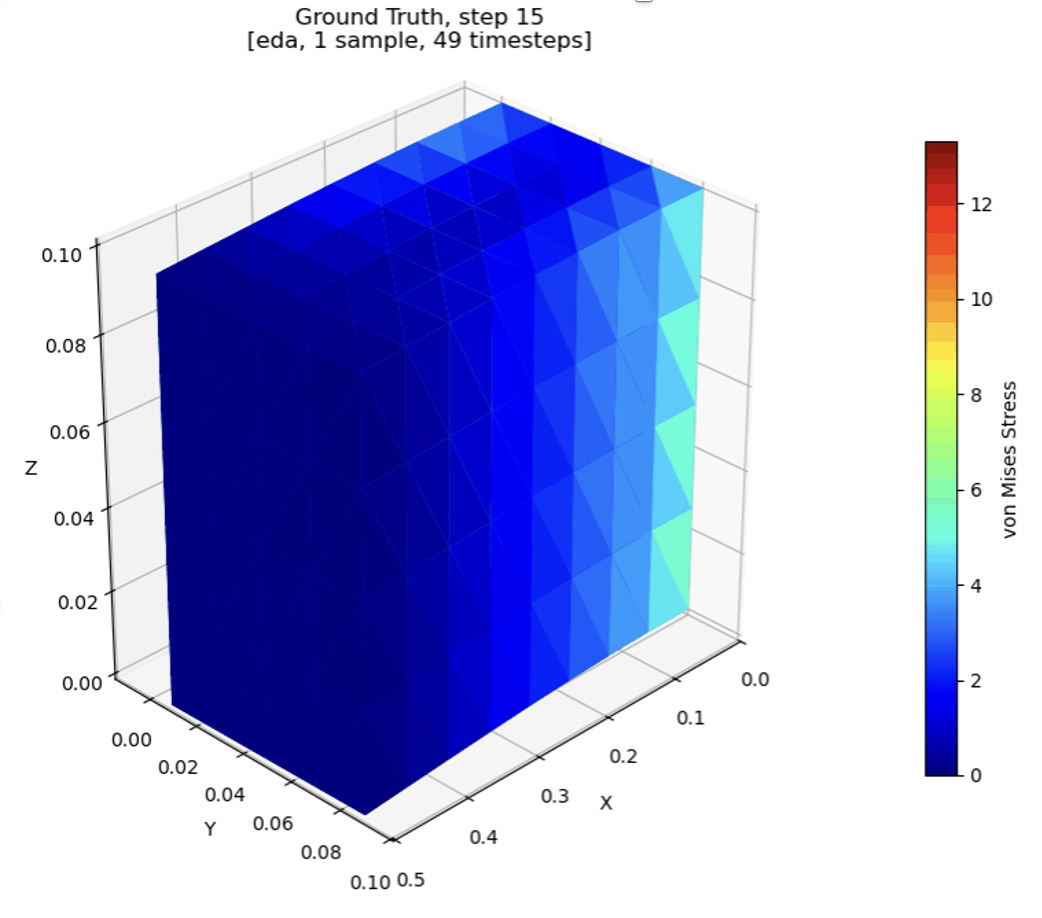
\includegraphics[width=0.4\linewidth]{beam_ground_truth.png}
    \caption{Example of beam deformed under traction.}
    \label{fig:placeholder}
\end{figure}

\subsection{Boundary loading and trajectories}

The forcing is a ramp followed by release. In the final presentation the traction is biaxial in the $y$ and $z$ directions:
\begin{equation}
    p(t) =
    \begin{cases}
        (0, f_y t/t_c, f_z t/t_c)^\top, & t\le t_c,\\
        0, & t>t_c,
    \end{cases}
    \qquad
    t_c = 0.2T_{\mathrm{sim}}.
    \label{eq:traction-ramp}
\end{equation}
Earlier dataset sweeps also considered single-axis, biaxial, and triaxial forces, and two geometry families: beams in which the length is bigger than the other dimensions, and beams without this constraint. The final setting focuses on a beam-like geometry because unconstrained geometries can produce many thick, nearly stationary trajectories, which makes the learning problem less informative. We focus on biaxial forces because, for application-driven reasons, we are not primarily interested in deformation along the $x$ axis. At the same time, biaxial loading is still more complex than single-axis loading. Still, due to multi-axial coupling, we have movement along the x axis.

Each trajectory has $50$ time steps over $T_{\mathrm{sim}}=4.0$, with the simulation parameters $\alpha_m=\alpha_f=0$ in the generalized-$\alpha$/Newmark notation. The mesh resolution is $8$ along length, $4$ along width, and $4$ along depth. The dataset contains about $1000$ trajectories, split into $80\%$ train, $10\%$ validation, and $10\%$ test. Validation samples stay inside the training ranges but use different parameter values; test samples are outside the training ranges and are therefore used as out-of-distribution (OOD) evaluation.

\subsection{Targets: acceleration and stress}

The simulator predicts acceleration and stress. There are two stress-target choices. The first predicts scalar von Mises stress,
\begin{equation}
    y_i = \left[a_i,\, \sigma_{\vM,i}\right],
\end{equation}
while the second predicts the full symmetric stress tensor, inspired by the fact that it could be more directly related to the underlying PDE and thus might avoid having to learn \eqref{eq:von-mises}:
\begin{equation}
    y_i = \left[a_i,\, \sigma_i\right],
    \qquad
    \sigma_i =
    \begin{bmatrix}
        \sigma_{xx} & \tau_{xy} & \tau_{xz}\\
        \tau_{xy} & \sigma_{yy} & \tau_{yz}\\
        \tau_{xz} & \tau_{yz} & \sigma_{zz}
    \end{bmatrix}_i.
\end{equation}
The von Mises scalar is computed from the stress components by
\begin{equation}
    \sigma_{\vM}=\biggl(
        \frac{(\sigma_{xx}-\sigma_{yy})^2
        +(\sigma_{yy}-\sigma_{zz})^2
        +(\sigma_{zz}-\sigma_{xx})^2
        +6(\tau_{xy}^2+\tau_{yz}^2+\tau_{xz}^2)}{2}
    \biggr)^{1/2}.
    \label{eq:von-mises}
\end{equation}
A key empirical outcome is that full stress tensor supervision is more useful than von Mises-only supervision, especially when combined with an auxiliary von Mises residual.

For scalar von Mises prediction, we applied a logarithmic transformation to the target and computed the loss in log-space. 

\subsection{Evaluation quantities}

The main rollout metric is the mean absolute position error averaged over nodes, coordinates, time steps, and trajectories. Single-step metrics are computed for acceleration and stress under teacher-forced inputs. As an additional global rollout metric, we use the volume error, which measures whether the predicted trajectory preserves the overall shape of the beam beyond local displacement accuracy.

\section{Methodology}
\label{sec:methodology}

\subsection{Learning framework}

The learning setup follows the GNS framework. At time $t$, the system state is represented as a graph with node features and edge features,
\begin{equation}
    X_t = \{x_{i,t}\}_{i=1}^N,
    \qquad
    G_t=(V,E,\{x_{i,t}\}_{i\in V},\{e_{ij,t}\}_{(i,j)\in E}).
\end{equation}
The input is a short history of states,
\begin{equation}
    \hat X_{t_0:t_K} = (X_{t_0},\hat X_{t_1},\ldots,\hat X_{t_K}),
\end{equation}
where teacher-forced training uses ground-truth histories and autoregressive inference uses previously predicted states. A learnable model $\phi_\theta$ predicts next-step target features:
\begin{equation}
    \hat Y_{t_K+1}=\phi_\theta(\hat X_{t_0:t_K}).
\end{equation}
An integrator then updates the full state:
\begin{equation}
    \hat X_{t_K+1}=\Integrator(\hat X_{t_0:t_K},\hat Y_{t_K+1}).
    \label{eq:simulator}
\end{equation}
For acceleration targets, the rollout implementation uses a second-order update of the form
\begin{equation}
    \hat v_{t+1}=v_t+\Delta t\,\hat a_t,
    \qquad
    \hat p_{t+1}=p_t+\Delta t\,v_t+\Delta t^2\hat a_t,
    \label{eq:rollout-integrator}
\end{equation}
with velocities and accelerations also recomputed from positions by finite differences for preprocessing and evaluation.

\subsection{Features}

A broad feature set was tested. Node features included clamping indicators, velocity, displacement $u_t=x_t-x_{\mathrm{rest}}$, force, current position, previous position, rest position, previous displacement, and norms such as $\norm{u_t}_2$, $\norm{f_t}_2$, $\norm{v_t}_2$, and $\norm{u_{t-1}}_2$. Edge features included relative displacement, relative velocity, relative force, current relative position, rest relative position, previous relative displacement, previous relative position, edge lengths, stretch ratios, and deformation-angle features such as
\begin{equation}
    \frac{\norm{x_{ij,t}}_2}{\norm{r_{ij}}_2+\varepsilon},
    \qquad
    \frac{r_{ij}}{\norm{r_{ij}}_2}\cdot \frac{x_{ij,t}}{\norm{x_{ij,t}}_2}.
\end{equation}
Here $x_{ij,t}=x_{j,t}-x_{i,t}$ and $r_{ij}=x_{\mathrm{rest},j}-x_{\mathrm{rest},i}$. Feature ablations showed that these hand-designed features are not decisive. They can help performance, but the dominant effects came from architecture, target choice, and noise.

\subsection{Training protocol}

Training uses teacher forcing with a mean absolute error objective (which, we found, performed better than a mean squared error objective) and Adam optimizer. Validation and testing are autoregressive rollouts, with the test set additionally out of distribution in force or geometry ranges. Sweeps were conducted on a reduced dataset of about $500$ trajectories. Section~\ref{subsec:main-arch-comparison} instead used the larger dataset. 

The best stress-target configuration used full stress tensor prediction plus a von Mises residual, with the two stress-related terms weighted equally.

\subsection{Architectures}

This section describes each architecture in a self-contained way and gives a compact system of equations. The goal is to expose the inductive bias each architecture imposes.

\subsubsection{MeshGraphNet}

MeshGraphNet is the local message-passing baseline. It fits naturally in the GNS framework, accepts edge features, and is a standard reference model for learned mesh-based physical simulation. Its inductive bias is local: information propagates through repeated message-passing steps along mesh edges. 

The model is an encoder--processor--decoder. Node and edge features are first embedded by MLP encoders. The processor then alternates edge updates and node updates. A version with mesh edges $E_M$ and optional special or ``world'' edges $E_W$ can be written as
\begin{equation}
\left\{
\begin{aligned}
    v_i^0 &= \epsilon_v(x_i), \\
    e_{ij}^{M,0}&=\epsilon_e^M(e_{ij}), \\
    e_{ij}^{W,0}&=\epsilon_e^W(e_{ij}),\\
    e_{ij}^{M,\ell+1}
    &= e_{ij}^{M,\ell}+\phi_E^{M,\ell}(e_{ij}^{M,\ell},v_i^\ell,v_j^\ell),
    && (i,j)\in E_M,\\
    e_{ij}^{W,\ell+1}
    &= e_{ij}^{W,\ell}+\phi_E^{W,\ell}(e_{ij}^{W,\ell},v_i^\ell,v_j^\ell),
    && (i,j)\in E_W,\\
    m_i^{M,\ell+1}&=\sum_{j:(i,j)\in E_M}e_{ij}^{M,\ell+1}, \\
    m_i^{W,\ell+1}&=\sum_{j:(i,j)\in E_W}e_{ij}^{W,\ell+1},\\
    v_i^{\ell+1}&=v_i^\ell+\phi_V^\ell(v_i^\ell,m_i^{M,\ell+1},m_i^{W,\ell+1}),
    && i\in V,\\
    \hat y_i&=\delta(v_i^L).
\end{aligned}
\right.
\label{eq:mgn}
\end{equation}
We have $E_W=\emptyset$. 
% The residual connections in the latent node and edge states help optimization, while shared MLPs preserve permutation equivariance over nodes.

\subsubsection{ClofNet}

ClofNet is an equivariant architecture based on complete local frames. It aims to separate invariant scalar information from equivariant vector information. The non-learnable part constructs a local frame $\mathcal F_{ij}$ for each edge, scalarizes equivariant quantities into coordinates in that frame, and later vectorizes learned scalar messages back into physical vectors. This gives an equivariance bias: if the entire system is rotated or translated, vector outputs rotate consistently and scalar outputs remain invariant.

Let $h_i^\ell$ denote invariant node features and $a_i^\ell$ an equivariant vector feature, such as acceleration. Let $\chi_i^\ell$ collect equivariant inputs such as displacement, velocity, acceleration, and force. A compact ClofNet layer is
\begin{equation}
\left\{
\begin{aligned}
    \mathcal F_{ij}^\ell &= \EquiFrame(u_i^\ell,u_j^\ell),\\
    s_{ij}^\ell &= \Scalarize(\chi_i^\ell,\chi_j^\ell,\mathcal F_{ij}^\ell),\\
    m_{ij}^\ell &= \phi_m^\ell(s_{ij}^\ell,h_i^\ell,h_j^\ell,e_{ij}),\\
    h_i^{\ell+1} &= \phi_h^\ell\left(h_i^\ell,\sum_{j\in\mathcal N(i)}m_{ij}^\ell\right),\\
    a_i^{\ell+1} &= a_i^\ell+\frac{1}{|\mathcal N(i)|}\sum_{j\in\mathcal N(i)}
    \Vectorize(m_{ij}^\ell,\mathcal F_{ij}^\ell),\\
    \hat a_i&=a_i^L,\qquad \hat\sigma_i=\delta_\sigma(h_i^L).
\end{aligned}
\right.
\label{eq:clofnet-vanilla}
\end{equation}
The project found that the vanilla form is unstable and not sufficiently expressive for this task. Several implementation and architectural changes improved behaviour: LayerNorm in MLPs, soft normalization with a small $\varepsilon$ rather than adding $1$ to norms, isotropic normalization of equivariant updates, using displacement rather than absolute position to build frames, and re-scalarizing at every layer.

Two message-passing variants were tested, while preserving equivariance. The \emph{nonlinear-message} variant feeds the previous message into the next edge MLP, enabling nonlinearities across message passing layers:
\begin{equation}
\left\{
\begin{aligned}
    m_{ij}^{\ell+1}&=\phi_m^\ell(s_{ij},h_i^\ell,h_j^\ell,e_{ij},m_{ij}^{\ell}),\\
    h_i^{\ell+1}&=\phi_h^\ell\left(h_i^\ell,\sum_{j\in\mathcal N(i)}m_{ij}^{\ell+1}\right),\\
    a_i^{\ell+1}&=a_i^\ell+\frac{1}{|\mathcal N(i)|}\sum_{j\in\mathcal N(i)}
    \Vectorize(m_{ij}^{\ell+1},\mathcal F_{ij}).
\end{aligned}
\right.
\label{eq:clofnet-nonlinear}
\end{equation}
The \emph{separate-message} variant uses different messages for velocity (or other equivariant features, e.g. displacement and force) and acceleration, and enforces equivariant updates for all the equivariant features, each using its own set of messages:
\begin{equation}
\left\{
\begin{aligned}
    m_{ij}^{a,\ell} &= \phi_{m,a}^\ell(s_{ij},h_i^\ell,h_j^\ell,e_{ij}), \\
    m_{ij}^{v,\ell} &= \phi_{m,v}^\ell(s_{ij},h_i^\ell,h_j^\ell,e_{ij}),\\
    h_i^{\ell+1}&=\phi_h^\ell\left(h_i^\ell,\sum_{j\in\mathcal N(i)}m_{ij}^{\ell}\right),\\
    v_i^{\ell+1}&=v_i^\ell+\frac{1}{|\mathcal N(i)|}\sum_{j\in\mathcal N(i)}\Vectorize(m_{ij}^{v,\ell},\mathcal F_{ij}),\\
    a_i^{\ell+1}&=a_i^\ell+\frac{1}{|\mathcal N(i)|}\sum_{j\in\mathcal N(i)}\Vectorize(m_{ij}^{a,\ell},\mathcal F_{ij})
        +\phi_v(h_i^{\ell+1})\odot v_i^{\ell+1}.
\end{aligned}
\right.
\label{eq:clofnet-separate}
\end{equation}
We were indeed able to enhance ClofNet performance by combining these two improvements, but we think its scalarization and vector update constraints may excessively limit expressivity in practice.

\subsubsection{Graph U-Net}

Graph U-Net is a hierarchical graph model. It pools nodes by a learnable score, applies graph convolutions on the coarsened graph, and unpools using saved indices. The intended bias is multi-scale: pooling should allow the model to summarize global or coarse interactions while preserving local detail through skip connections.

The graph pooling operation at layer $\ell$ can be summarized as
\begin{equation}
\left\{
\begin{aligned}
    y &= X^\ell p^\ell/\norm{p^\ell},\\
    \mathrm{idx} &= \rank(y,k),\\
    \tilde y &= \sigma(y(\mathrm{idx})),\\
    \tilde X^\ell &= X^\ell(\mathrm{idx},:),\\
    A^{\ell+1} &= A^\ell(\mathrm{idx},\mathrm{idx}),\\
    X^{\ell+1} &= \tilde X^\ell \odot (\tilde y\mathbf 1_C^\top).
\end{aligned}
\right.
\label{eq:graphunet-pool}
\end{equation}
The convolution used in the encoder/decoder stages is of the GCN form
\begin{equation}
    X_{\ell+1}=\sigma\left(\hat D^{-1/2}\hat A\hat D^{-1/2}X_\ell W_\ell\right).
    \label{eq:gcn}
\end{equation}
In this project Graph U-Net was unable to fit the beam dynamics, as can be seen in Appendix F. A plausible explanation, consistent with the literature on graph convolutions for physical simulation, is that repeated normalized graph convolution acts as a low-pass filter and suppresses the high-frequency ``wobbly'' behavior that is essential in the beam problem. Moreover, it may suffer from the absence of edge features.

\subsubsection{GATv2}

GATv2 introduces learned local attention weights on graph neighborhoods. It keeps the mesh-local receptive field of a GNN, but replaces uniform or purely MLP-based aggregation by adaptive neighbor weights. The relevant bias is therefore local attention rather than global attention.

For head $k$ in layer $\ell$, GATv2 computes
\begin{equation}
\left\{
\begin{aligned}
    z_i^{(\ell,k)} &= W^{(\ell,k)}h_i^{(\ell)},\\
    e_{ij}^{(\ell,k)}&=(a^{(\ell,k)})^\top
    \operatorname{LeakyReLU}\left(W^{(\ell,k)}[h_i^{(\ell)}\Vert h_j^{(\ell)}]\right),\\
    \alpha_{ij}^{(\ell,k)}&=\frac{\exp(e_{ij}^{(\ell,k)})}{\sum_{r\in\mathcal N(i)}\exp(e_{ir}^{(\ell,k)})},\\
    m_{j\to i}^{(\ell,k)}&=\alpha_{ij}^{(\ell,k)}z_j^{(\ell,k)},\\
    s_i^{(\ell,k)}&=\sum_{j\in\mathcal N(i)}m_{j\to i}^{(\ell,k)},\\
    h_i^{(\ell+1)}&=\big\Vert_{k=1}^{K_\ell}\sigma(s_i^{(\ell,k)}).
\end{aligned}
\right.
\label{eq:gatv2}
\end{equation}
GATv2 can weight different neighbors differently, partially addressing the shared-weight bottleneck of message passing. However, because attention is still restricted to local mesh neighborhoods, it did not recover the benefits of global attention in this task, see Appendix F.

\subsubsection{Transolver}

Transolver is a transformer-style PDE solver that avoids full $O(N^2)$ node-node attention by routing nodes into a smaller set of learned physical tokens or slices. Its inductive bias is global but structured: nodes that are far apart in mesh topology can communicate through the same token if their learned routing weights assign them to related physical states.

Let $x_i^\ell\in\R^C$ be node features and let $M\ll N$ be the number of tokens. The physics-attention layer can be summarized as
\begin{equation}
\left\{
\begin{aligned}
    x_i^0 &= \operatorname{Linear}(\concat(g_i,u_i)),\\
    w_i &= \softmax(\operatorname{Project}(x_i)),\qquad i=1,\ldots,N,\\
    z_j &= \frac{\sum_{i=1}^N w_{i,j}x_i}{\sum_{i=1}^N w_{i,j}},
    \qquad j=1,\ldots,M,\\
    q,k,v &= \operatorname{Linear}(z),\\
    z' &= \softmax\left(\frac{qk^\top}{\sqrt C}\right)v,\\
    x_i' &= \sum_{j=1}^M w_{i,j}z_j',\qquad i=1,\ldots,N.
\end{aligned}
\right.
\label{eq:transolver-attn}
\end{equation}
The complete block uses the standard transformer residual structure,
\begin{equation}
\left\{
\begin{aligned}
    \hat x^\ell &= \PhysicsAttn(\LayerNorm(x^{\ell-1}))+x^{\ell-1},\\
    x^\ell &= \FeedForward(\LayerNorm(\hat x^\ell))+\hat x^\ell,
    \qquad \ell=1,\ldots,L.
\end{aligned}
\right.
\label{eq:transolver-block}
\end{equation}
Transolver was the strongest overall architecture in the final results.

\subsection{Topology augmentation}

To separate architectural globality from graph-connectivity globality, the project tested several edge augmentations on top of the mesh graph:
\begin{equation}
    E_{\mathrm{aug}}=E_{\mathrm{mesh}}\cup E_{k\text{-hop}}\cup E_{\mathrm{wall}}\cup E_{\mathrm{rand}}(p).
    \label{eq:edge-aug}
\end{equation}
Here $E_{k\text{-hop}}$ adds connections between nodes within $k$ mesh hops, $E_{\mathrm{wall}}$ adds special edges to wall-clamped nodes, and $E_{\mathrm{rand}}(p)$ samples random spatial skip edges online or offline. Fully connected graphs were considered conceptually, but were computationally infeasible in this setting: the edge count grows as $O(N^2)$ and, for example for MGN, one epoch took about one hour. In Appendix F, we can see that the best performing topology augmentation technique was random edge augmentation.

\subsection{Noise and target correction}

Teacher forcing creates exposure bias: during training, the model sees clean states; during rollout, it sees its own imperfect predictions, and error compounds over time. The most successful training bias was online noising with target correction. Perturbations are resampled each epoch rather than fixed offline:
\begin{equation}
    \tilde p_t=p_t+\xi_t,
    \qquad
    \xi_t\sim\mathcal N(0,\sigma_n^2 I).
\end{equation}

A possible explanation for why online noising performs better is that it is more closely connected to stability notions for dynamical systems, such as those arising in ODEs. By repeatedly perturbing nearby states and correcting the target, the model is encouraged to learn a local recovery field around the true trajectory, rather than only fitting the trajectory itself.

In contrast, offline noising is theoretically closer to learning a fixed mapping of the form $\tilde{x} \mapsto y$: each perturbed input is always associated with the same target, and the model may never observe the corresponding clean feature, or nearby variants of the same feature, during training. Nevertheless, offline noising can still be beneficial. Across the dataset (the various timesteps and trajectories), many nodes lie close to one another in space, and their independent perturbations might create an effect similar to online noising. 
% Thus, even fixed offline perturbations can expose the model to nearby off-manifold states, although less flexibly than online noising.

The target is then corrected so the model learns to recover from nearby off-manifold states. For the integrator in~\eqref{eq:rollout-integrator}, two natural corrected accelerations are
\begin{equation}
    \tilde a_t^P=\frac{p_{t+1}-\tilde p_t-\Delta t\,\tilde v_t}{\Delta t^2},
    \qquad
    \tilde a_t^V=\frac{v_{t+1}-\tilde v_t}{\Delta t}.
\end{equation}
The first makes the next position correct, while the second makes the next velocity correct. For a second-order system both cannot generally be satisfied exactly after perturbing the input, so the project used
\begin{equation}
    \tilde a_t = \gamma\tilde a_t^P+(1-\gamma)\tilde a_t^V.
    \label{eq:noise-correction}
\end{equation}
The best final noise configuration used online noising, magnitude $5\cdot 10^{-4}$, and $\gamma=0.01$.

\subsection{Physics-motivated residuals}

Several residuals were tested as soft penalties rather than hard constraints. The curvature residual penalizes excessive surface bending beyond the maximum observed in training. If two adjacent surface triangles have normals $\hat n_L$ and $\hat n_R$, then
\begin{equation}
    \theta=\arccos\left(\operatorname{clamp}(\hat n_L\cdot\hat n_R,-1+\varepsilon,1-\varepsilon)\right),
    \qquad
    \mathcal R_{\mathrm{curv}}=\frac{1}{|\mathcal S|}\sum_{e\in\mathcal S}\relu(\theta_e-\theta_{\max}).
\end{equation}
The volume residual penalizes global drift,
\begin{equation}
    \mathcal R_{\mathrm{vol}}=\abs{V(\hat P_{t+1})-V(P_{t+1})},
\end{equation}
and the von Mises residual for full-stress predictions is
\begin{equation}
    \mathcal R_{\vM}=\norm{\sigma_{\vM}(\hat\sigma)-\sigma_{\vM}(\sigma)}_1.
\end{equation}
The residual experiments suggested that the volume drift and angle drift penalizations can regularize particular failure modes, but they were not game-changers under one-step teacher-forced training.

\section{Results}
\label{sec:results}

\subsection{Main architecture comparison}\label{subsec:main-arch-comparison}

Table~\ref{tab:main-results} summarizes the best final results for Transolver, MeshGraphNet, and ClofNet. All metrics are MAE, averaged over nodes for a given time step, then over time steps in a trajectory, and finally over trajectories. 

\begin{table}[ht]
\centering
\caption{Best reported validation and OOD test results. Lower is better. Transolver: hidden dimension 312, 7 Transolver blocks, 15 heads, resulting in $\approx 8$ million parameters. MGN: hidden dimension of 256, 15 message passing layers, resulting in an $\approx 7.5$ million parameters.}
\label{tab:main-results}
\begin{tabular}{llccc}
\toprule
Split & Metric & Transolver & MeshGraphNet & ClofNet \\
\midrule
Validation & Rollout position & $2.4\times10^{-3}$ & $8.4\times10^{-3}$ & $5.4\times10^{-3}$ \\
Validation & Single-step stress tensor & $6.8\times10^{-3}$ & $2.1\times10^{-2}$ & $2.8\times10^{-1}$ \\
Validation & Volume rollout & $4.8\times10^{-5}$ & $3.0\times10^{-4}$ & $5.5\times10^{-4}$ \\
\midrule
Test (OOD) & Rollout position & $8.8\times10^{-3}$ & $1.7\times10^{-4}$ & $1.2\times10^{-1}$ \\
Test (OOD) & Single-step stress tensor & $3.0\times10^{-4}$ & $8.0\times10^{-4}$ & $7.0\times10^{-1}$ \\
Test (OOD) & Volume rollout & $3.8\times10^{-2}$ & $6.0\times10^{-2}$ & $4.3$ \\
\bottomrule
\end{tabular}
\end{table}

Transolver is best on position rollout, stress tensor prediction, and volume. On OOD test, MeshGraphNet obtains the smallest position rollout error, but Transolver remains best on stress and volume. 
For all architectures, including Graph U-Net and MGN, extended sweeps were conducted, resulting in more than 150 WandB runs. The results reported here are with full stress tensor targets.
Further results are shown in Appendix F.

\begin{figure}[h!]
    \centering
    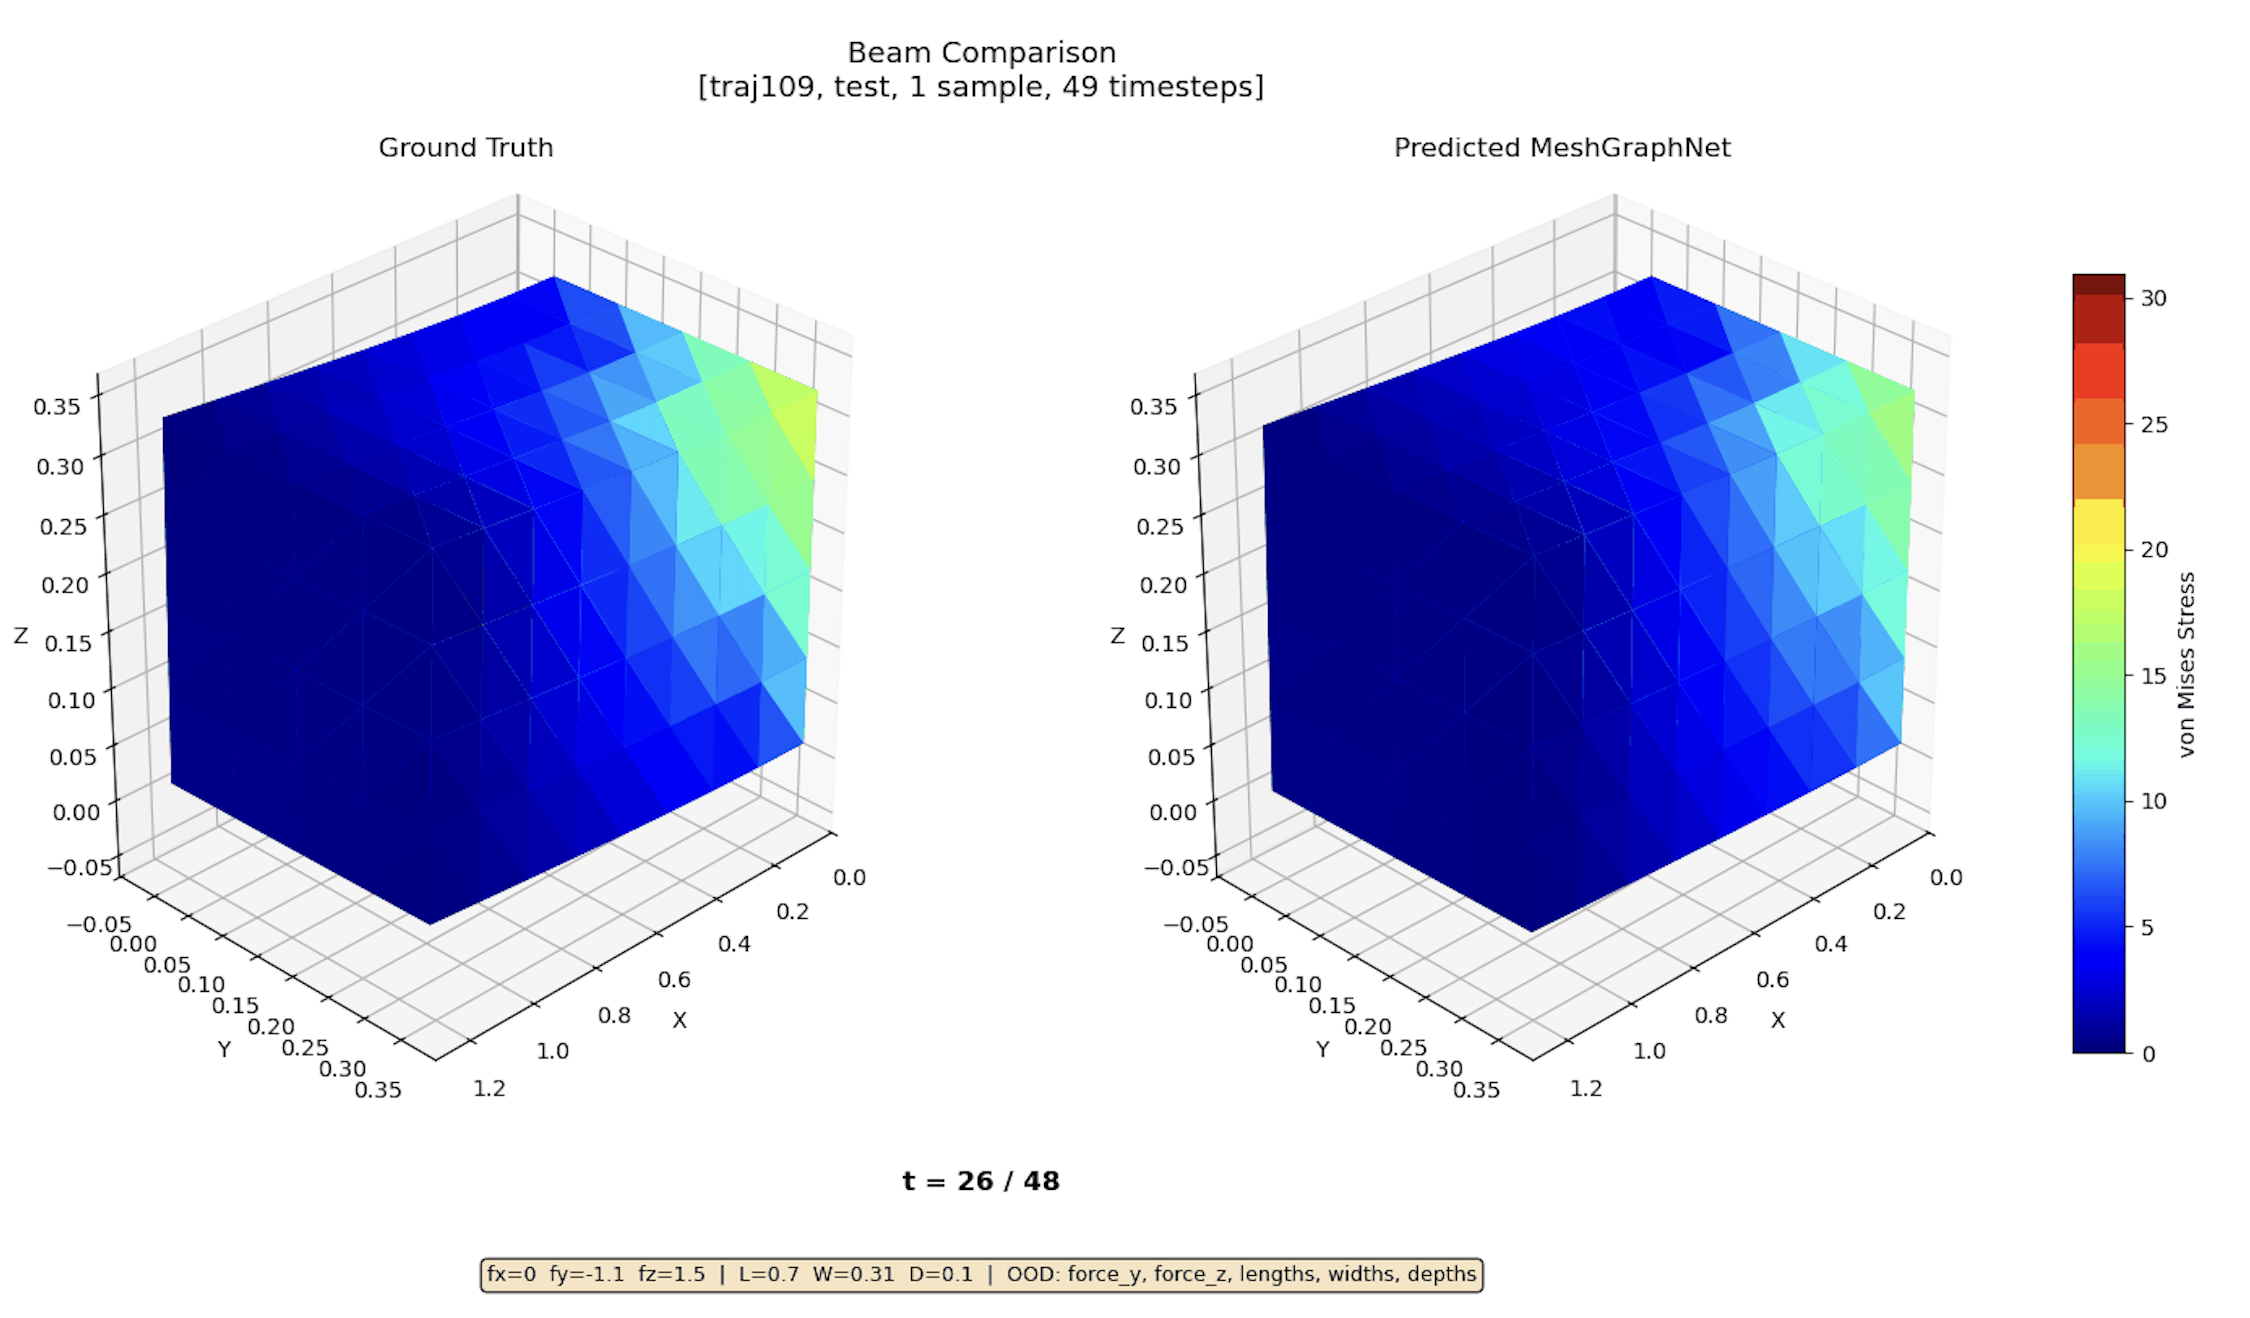
\includegraphics[width=0.5\linewidth, trim={0cm 0cm 0cm 3.6cm}, clip]{img/trans_beam_1.png}
    \caption{Example of Transolver rollout beam prediction (right) vs ground truth (left). Test set.}
    \label{fig:placeholder}
\end{figure}

\subsection{Interpretation of architectural biases}

The final ranking of architectures is
\begin{equation}
    \text{Transolver} > \text{MeshGraphNet} > \text{ClofNet} > \text{GATv2}\approx\text{Graph U-Net}.
\end{equation}

The beam dynamics require both local elastic consistency and global communication. MeshGraphNet has a strong local bias and fits the data, but it must propagate global information through many message-passing layers. ClofNet adds a geometric equivariance bias, but its scalarization and equivariant-update constraints appear to limit expressivity for acceleration and stress. GATv2 uses attention, but only inside local neighborhoods, so it does not provide the same global context as Transolver. Graph U-Net introduces hierarchy, but its graph-convolution (coupled with the absence of edge features) appears too smoothing for high-frequency dynamics.

Transolver's advantage is that it is global without requiring a fully connected graph. The physical-token representation lets distant nodes exchange information through learned slices. Attention visualizations in Appendix F show different attention patterns for clamped-wall nodes, tip nodes, and middle-beam nodes. 

\subsection{Stress target and qualitative behavior}

Full stress tensor supervision improves learning compared with von Mises-only supervision. Predicting only von Mises collapses tensorial information into a scalar, losing shear and principal-direction structure that is useful for the dynamics. The best target design predicts the full tensor and also penalizes the von Mises scalar computed from it. 

Qualitatively, Transolver produced the best stress scatter plots on the large test setting, while MGN produced plausible deformation rollouts and strong OOD position behavior. ClofNet was visually unstable in its vanilla form and improved only after implementation changes and message variants. 

To the best of our knowledge, this change of perspective, i.e. predicting the full stress tensor and then obtaining the von Mises stress instead of directly predicting the von Mises stress, is novel, at least in papers within our autoregressive GNS framework for mechanics.

\section{Ablations}
\label{sec:ablations}

\subsection{Locality versus globality through edge augmentation}

The first locality/globality question was whether one can make a local message-passing GNN more global by adding edges. Table~\ref{tab:edge-aug} summarizes the reported MGN edge augmentation results. The table shows both improvements and instabilities.

\begin{table}[H]
\centering
\caption{Edge augmentation ablation for MGN. Lower is better. Some $k$-hop variants improved stress but produced catastrophic volume rollouts. Random edge augmentation performs the best.}
\label{tab:edge-aug}
\resizebox{\textwidth}{!}{%
\begin{tabular}{llcccccccc}
\toprule
Split & Metric & Default & Random 3\% & Wall & 2-hop & 3-hop \#2 & 3-hop+wall \#2 & Random 20\% \#2 & 2-hop \#2 \\
\midrule
Val & Volume rollout & $3.5\mathrm{e}{-3}$ & $2.6\mathrm{e}{-4}$ & $2.8\mathrm{e}{-3}$ & $2.3$ & $1.7\mathrm{e}{-3}$ & $4.0\mathrm{e}{-4}$ & $1.6\mathrm{e}{-4}$ & $135$ \\
Val & Position rollout & $8.0\mathrm{e}{-3}$ & $7.6\mathrm{e}{-3}$ & $7.4\mathrm{e}{-3}$ & $2.6\mathrm{e}{-2}$ & $1.2\mathrm{e}{-2}$ & $7.7\mathrm{e}{-3}$ & $3.8\mathrm{e}{-3}$ & $1.0\mathrm{e}{-1}$ \\
Val & Single-step stress & $1.6\mathrm{e}{-1}$ & $4.6\mathrm{e}{-2}$ & $1.5\mathrm{e}{-1}$ & $4.7\mathrm{e}{-2}$ & $1.4\mathrm{e}{-1}$ & $9.1\mathrm{e}{-2}$ & $4.8\mathrm{e}{-2}$ & $5.9\mathrm{e}{-2}$ \\
\midrule
Test & Volume rollout & $8.8\mathrm{e}{-3}$ & $1.7\mathrm{e}{-1}$ & $5.5\mathrm{e}{-3}$ & $181$ & $25$ & $9.6\mathrm{e}{-4}$ & $3.8\mathrm{e}{-4}$ & $677$ \\
Test & Position rollout & $1.6\mathrm{e}{-2}$ & $2.5\mathrm{e}{-3}$ & $1.7\mathrm{e}{-2}$ & $1.2\mathrm{e}{-1}$ & $2.6\mathrm{e}{-1}$ & $1.4\mathrm{e}{-2}$ & $7.5\mathrm{e}{-3}$ & $2.0\mathrm{e}{-1}$ \\
Test & Single-step stress & $4.5\mathrm{e}{-1}$ & $3.0\mathrm{e}{-1}$ & $4.5\mathrm{e}{-1}$ & $2.0\mathrm{e}{-1}$ & $1.9\mathrm{e}{-1}$ & $1.5\mathrm{e}{-1}$ & $1.3\mathrm{e}{-1}$ & $2.0\mathrm{e}{-1}$ \\
\bottomrule
\end{tabular}}
\end{table}

The main lesson is that edge augmentation is not equivalent to architectural globality. Random $20\%$ edges and $3$-hop plus wall edges can improve volume or stress metrics, but some $2$-hop and $3$-hop variants produce excessive volume drift. Adding edges also makes the dataset graph larger and training slower; for MGN this is particularly costly because edge features are part of the processor. Fully connected message passing was not practical.

This suggests a useful distinction:
\begin{itemize}[leftmargin=1.3em]
    \item \emph{Architectural globality}, as in Transolver, controls how global information is compressed and routed.
    \item \emph{Connectivity globality}, as in edge augmentation, simply gives a local message-passing architecture more neighbors, without necessarily providing a stable way to use them.
\end{itemize}
For this beam task, architectural globality was more reliable. Detailed results for the sweeps can be found in Appendix F. 

\subsection{Noising and exposure bias}

Online noising was the most important training bias. Fixed offline noise can be memorized as a new deterministic input distribution, whereas online noise forces the model to learn recovery behavior around the clean trajectory manifold. The best configuration used online noising, magnitude $5\cdot 10^{-4}$, and target-correction parameter $\gamma=0.01$.

This directly addresses exposure bias. During rollout the model sees states perturbed by its own errors. Online noising exposes the model during training to analogous perturbations and teaches it to return to the ground-truth trajectory. The effect was observed across architectures. Detailed results for the sweeps can be found in Appendix F.

\subsection{Residual losses}

Residual penalties were conceptually appealing but empirically modest. Curvature penalties had to be weighted far below the main loss to avoid dominating optimization. Volume penalties had magnitudes closer to the main loss and could reduce drift, but did not fundamentally change the ranking of architectures. The additional von Mises residual was the most useful residual because it complemented full tensor stress supervision rather than imposing an independent geometric constraint.

A likely explanation is the training regime: residuals are applied under teacher forcing, but the worst physical errors appear during rollout after compounding model errors. Therefore residuals on single-step predictions do not fully solve autoregressive drift. A future extension would apply residuals to multi-step unrolled training windows. 

Detailed results for the sweeps can be found in Appendix F.

\subsection{Target ablations}

The stress target ablation yielded the following result:
\begin{equation}
    \text{full stress tensor + von Mises residual} > \text{full stress tensor only} > \text{von Mises only}.
\end{equation}
Exponentiating von Mises predictions only at final evaluation, rather than computing the loss directly in original stress space, did not improve results. 
Detailed results for the sweeps can be found in Appendix F.

\subsection{Feature and dataset ablations}

Hand-designed features such as stretch ratio and deformation angle did not produce major gains. 
Dataset ablations showed that the small dataset of around $200$ trajectories performed poorly even with noising. The ``allgeoms'' setting produced lower rollout errors for some metrics, but this likely reflected many thick geometries with little motion rather than genuinely better generalization. The final benchmark therefore uses a geometry distribution that remains beam-like.

\subsection{Graph U-Net and GATv2 failures}

Graph U-Net and GATv2 were unable to fit the data well enough to be competitive. For Graph U-Net, the likely issue is excessive smoothing: graph convolution and pooling can suppress high-frequency oscillations. Moreover, they do not accept edge features. For comparison, we also ran an ablation in which MGN was trained without edge features (omitted for the sake of brevity). Its performance degraded as well, suggesting that the absence of edge features may also contribute to the poor results. For GATv2, the issue is not the absence of attention, but the locality of attention. The final conclusion is therefore: attention is useful, but local message-passing attention is not enough for this beam problem. Global attention through physical tokens was substantially more effective. Detailed results can be found in Appendix F.

\subsection{Computational considerations}

The project code implements a full pipeline: finite element dataset generation, preprocessing and exploratory analysis, training, evaluation, and integration with \texttt{WandB}, \texttt{Hydra}, \texttt{Lightning}, and \texttt{Optuna}. A fixed mesh produces stable computation graphs, making compilation beneficial. For MeshGraphNet, \texttt{torch.compile} gave about a $15$--$20\%$ speedup in the profiling experiments. ClofNet also benefits from \texttt{torch.compile}. Besides \texttt{torch.compile}, JIT compilation was also used for online data-processing components such as the online noising procedure. If further optimization is required, the non-learnable scalarization part of ClofNet could be JIT compiled.

Transolver was not only more accurate overall, but also faster per epoch in the reported configuration. MGN and ClofNet scale worse with edge augmentation because their processors explicitly carry edge features through message passing.

\section{Conclusions}\label{sec:conclusions}

The project leads to seven main conclusions. 

\begin{enumerate}[leftmargin=1.5em]
    \item \textbf{Globality helps, but how it is introduced matters.} Transolver's global physical-token attention outperformed purely local MeshGraphNet on most validation metrics and on OOD stress/volume. Edge augmentation did improve performance, but in a minor way.
    \item \textbf{Attention is not all that is needed.} Local attention through GATv2 did not match global attention through Transolver. The important bias is not attention by itself, but global communication with a useful over-squashing avoidance mechanism.
    \item \textbf{Online noising is the strongest training bias.} It directly addresses rollout exposure bias and improves robustness across architectures.
    \item \textbf{Residuals are secondary regularizers.} Volume, curvature, and von Mises residuals can help specific quantities, but simple one-step residual training does not by itself solve rollout drift.
    \item \textbf{Full stress is a better target than von Mises alone.} Tensor supervision preserves directional and shear information. A derived von Mises residual is useful as an auxiliary term and it's more accurate than directly predicting von Mises stress.
    \item \textbf{Equivariance alone is insufficient.} ClofNet encodes an attractive physical prior, but its scalarization and vector-update constraints limited expressivity on this task.
    \item \textbf{Hierarchical smoothing can be harmful for high-frequency dynamics.} Graph U-Net struggled, consistent with the view that graph convolution can act as a low-pass filter.
\end{enumerate}
\noindent
Taken together, these results suggest that less restrictive inductive biases can improve performance. Transolver performs best overall, likely because its global attention mechanism allows long-range communication without forcing information to propagate through many local message-passing layers, as the attention visualization in Appendix F shows. At the same time, message-passing architectures require sufficient depth, or additional connectivity, to cover the whole mesh.

In terms of architecture, a concise final ranking is
\begin{equation}
    \boxed{\text{Transolver} > \text{MeshGraphNet} > \text{ClofNet (Variants)} > \text{GATv2}\approx\text{Graph U-Net}.}
\end{equation}

\section{Future work}\label{sec:futurework}
The most promising next directions are exposure-bias mitigation and scaling. First, the analogy with language modeling suggests masked pretraining and multi-step post-training: train the model not only to predict a one-step target from clean histories, but also to recover missing/noisy states and to optimize short unrolled rollouts. Second, the benchmark should be scaled to larger meshes and more varied topologies to test whether the conclusions persist when resolution and geometry change. Third, future models should combine equivariance with globality, for example by routing equivariant representations through global tokens or by adding attention to local-frame architectures. There are also some further improvements that can be made to ClofNet. Finally, stronger physics-informed training should apply residuals on unrolled trajectories, not only teacher-forced one-step predictions, to really benefit from the residuals, since metrics such as volume drift and wrinkly geometries artifacts become more noticeable.

\subsection*{Use of AI Tools}

AI tools were used to support parts of the code, including plotting, debugging, JIT compilation, and selected code modifications. 

% --- Bibliography ---
\bibliographystyle{amsplain}
\begin{thebibliography}{99}

\bibitem{learnable_physics_engines}
P. W. Battaglia, R. Pascanu, M. Lai, D. J. Rezende, and K. Kavukcuoglu,
\textit{Interaction networks for learning about objects, relations and physics},
Advances in Neural Information Processing Systems, 29, 2016.

\bibitem{hamiltonian_graph_networks}
A. Sanchez-Gonzalez, V. Bapst, K. Cranmer, and P. Battaglia,
\textit{Hamiltonian graph networks with ODE integrators},
arXiv:1909.12790, 2019.

\bibitem{gns}
A. Sanchez-Gonzalez, J. Godwin, T. Pfaff, R. Ying, J. Leskovec, and P. Battaglia,
\textit{Learning to simulate complex physics with graph networks},
arXiv:2002.09405, 2020.

\bibitem{mgn}
T. Pfaff, M. Fortunato, A. Sanchez-Gonzalez, and P. Battaglia,
\textit{Learning mesh-based simulation with graph networks},
arXiv:2010.03409, 2020.

\bibitem{gnss_structural}
A. Lucchetti, F. Cadini, M. Giglio, and L. Lomazzi,
\textit{Graph Network-based Structural Simulator: Graph Neural Networks for Structural Dynamics},
arXiv:2510.25683, 2025.

\bibitem{stiffened_panels}
Y. Cai and J. Jelovica,
\textit{Efficient graph representation in graph neural networks for stress predictions in stiffened panels},
Thin-Walled Structures, 203, 112157, 2024.

\bibitem{gnn_accelerated_simulation}
C. Jiang and N.-Z. Chen,
\textit{Graph Neural Networks (GNNs) based accelerated numerical simulation},
Engineering Applications of Artificial Intelligence, 123, 106370, 2023.

\bibitem{learning_based_fem}
J. Shi, F. Lin, and W. Rao,
\textit{Learning-Based Finite Element Methods Modeling for Complex Mechanical Systems},
arXiv:2409.00160, 2024.

\bibitem{mesh_gnn_pdes}
R. J. Gladstone, H. Rahmani, V. Suryakumar, H. Meidani, M. D'Elia, and A. Zareei,
\textit{Mesh-based GNN surrogates for time-independent PDEs},
Scientific Reports, 14, 3394, 2024.

\bibitem{gcn}
T. N. Kipf and M. Welling,
\textit{Semi-supervised classification with graph convolutional networks},
International Conference on Learning Representations, 2017.

\bibitem{gat}
P. Velickovic, G. Cucurull, A. Casanova, A. Romero, P. Lio, and Y. Bengio,
\textit{Graph attention networks},
arXiv:1710.10903, 2017.

\bibitem{gatv2}
S. Brody, U. Alon, and E. Yahav,
\textit{How attentive are graph attention networks?},
arXiv:2105.14491, 2021.

\bibitem{graphunet}
H. Gao and S. Ji,
\textit{Graph U-Nets},
arXiv:1905.05178, 2019.

\bibitem{bsms_gnn}
Y. Cao, M. Chai, M. Li, and C. Jiang,
\textit{Efficient learning of mesh-based physical simulation with bi-stride multi-scale graph neural network},
Proceedings of the 40th International Conference on Machine Learning, Proceedings of Machine Learning Research, 202, 3541--3558, 2023.

\bibitem{multigrid_self_attention}
P. Garnier, J. Viquerat, and E. Hachem,
\textit{Multi-grid graph neural networks with self-attention for computational mechanics},
Physics of Fluids, 37(8), 087140, 2025.

\bibitem{training_transformers_mesh}
P. Garnier, V. Lannelongue, J. Viquerat, and E. Hachem,
\textit{Training Transformers for Mesh-Based Simulations},
arXiv:2508.18051, 2025.

\bibitem{transolver}
H. Wu, H. Luo, H. Wang, J. Wang, and M. Long,
\textit{Transolver: A fast transformer solver for PDEs on general geometries},
arXiv:2402.02366, 2024.

\bibitem{egnn}
V. G. Satorras, E. Hoogeboom, and M. Welling,
\textit{E(n) equivariant graph neural networks},
Proceedings of the 38th International Conference on Machine Learning, Proceedings of Machine Learning Research, 139, 9323--9332, 2021.

\bibitem{clofnet}
W. Du, H. Zhang, Y. Du, Q. Meng, W. Chen, B. Shao, T.-Y. Liu, and L. Wang,
\textit{SE(3) equivariant graph neural networks with complete local frames},
Proceedings of Machine Learning Research, 162, 2022. Available at
\url{https://proceedings.mlr.press/v162/du22e/du22e.pdf}.

\end{thebibliography}

\clearpage

\section*{Appendix A: ClofNet details}

We wrote two diagnostic tests for investigating the equivariance behaviour of ClofNet's local-frame scalarization. 

The first test (Figure~\ref{fig:clof_test1}) constructs a beam-like lattice and compares
selected directed edges. In the first case, the two edges are obtainable from each other by a pure translation of both endpoints; in the second case, the two edges are oblique,
non-parallel, and non-orthogonal. For each directed edge, the test builds the ClofNet frame
\[
a_{ij} = \frac{x_i - x_j}{\|x_i - x_j\|}, \qquad
b_{ij} = \frac{x_i \times x_j}{\|x_i \times x_j\|}, \qquad
c_{ij} = a_{ij} \times b_{ij},
\]
after centroid-centering the node coordinates, and projects both endpoints onto this frame. The test asserts that every constructed frame is numerically orthonormal and right-
handed, and prints the endpoint scalarization coefficients for comparison.

The second test (Figure~\ref{fig:clof_test2}) applies the same scalarization to a whole lattice mesh. It builds a set of undirected lattice edges, duplicates them into both directed orders, then compares the
scalarization coefficients before and after applying a deterministic global rotation and translation to the entire mesh. Both meshes are centralized before constructing the local frames, and edges with degenerate cross products are skipped. 

\begin{figure}[H]
    \centering
    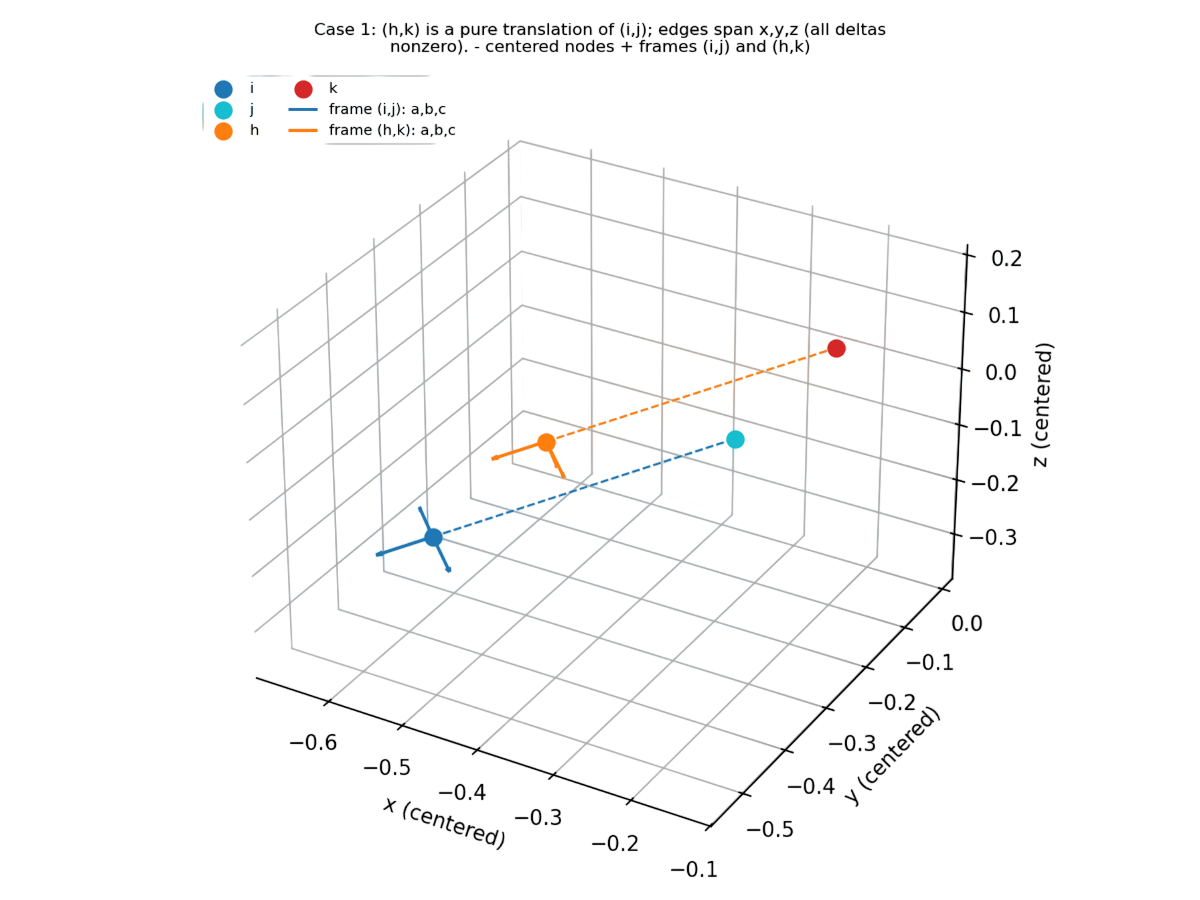
\includegraphics[width=0.5\linewidth]{test_clofnet.png}
    \caption{Test 1: as it can be seen, the local frames produced by the two pairs of nodes are indeed different. This is because SE(3)-equivariance is ensured only globally, not on any pair of nodes.}
        \label{fig:clof_test1}
\end{figure}

\begin{figure}[H]
    \centering
    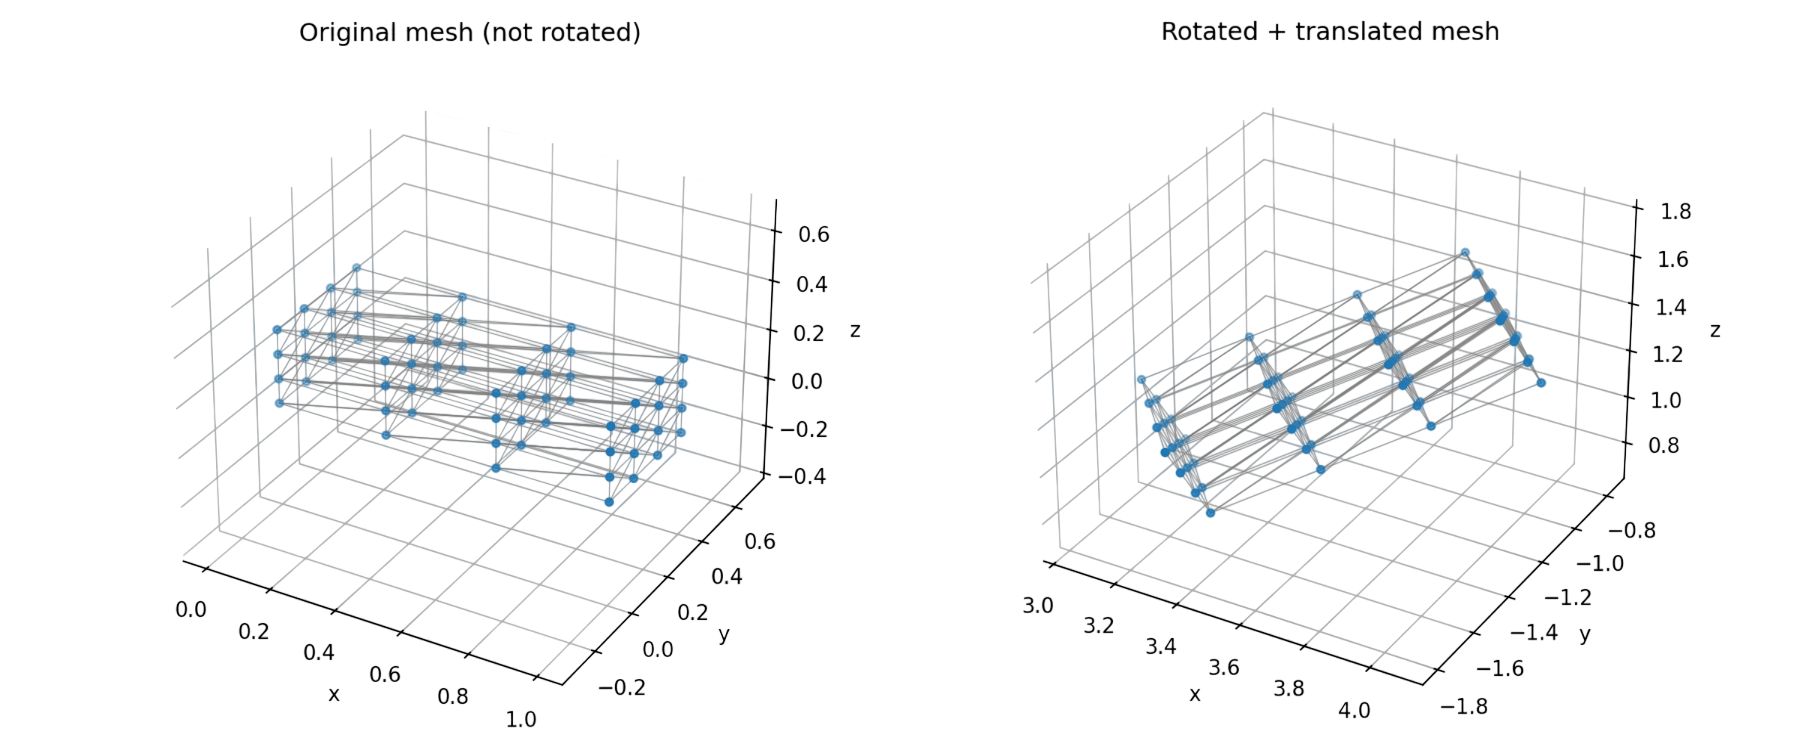
\includegraphics[width=0.8\linewidth]{test_clof_global.png}
    \caption{Test 2: ``global equivariance'', meaning the same rotation and translation is applied to the whole mesh.}
    \label{fig:clof_test2}
\end{figure}

\section*{Appendix B: interleaving MGN with GAT}

We also tested a hybrid message-passing architecture that interleaves MGN layers with occasional GAT layers. The motivation was that, although GAT alone was unable to fit the data, attention layers might still improve MGN by preserving its message-passing expressivity while reducing over-squashing through more adaptive aggregation. We tried one attention layer every 2 and 4 MGN layers: empirically, this architecture performed worse than the standard MGN baseline. We do not report results for brevity.

\section*{Appendix C: Interpretation of the PDE terms}

The different terms in~\eqref{eq:pde} have the standard interpretation of a damped linear-elasticity model. The term $\rho \ddot u$ is the inertial or mass contribution, while $\eta_m\rho \dot u$ is mass-proportional damping. The divergence of $\sigma(u)$ gives the internal elastic restoring force, and the additional term involving $\eta_k\sigma(\dot u)$ corresponds to stiffness-proportional damping. In the constitutive law, the trace term $\lambda\tr(\varepsilon(u))I$ models volumetric compression, while the $2\mu\varepsilon(u)$ term captures shear deformation.

\section*{Appendix D: Dataset}

The unconstrained-geometry setting is still conceptually interesting because it is less biased toward beam-like shapes. However, in the generated dataset it produced many thick and nearly stationary trajectories, making the learning problem less informative. A better version of this experiment would require explicit dataset balancing, so that the broader geometry distribution does not collapse into many low-motion samples.

\section*{Appendix E: Related Work}\label{app:related-work}

\noindent
We review some of the related literature.

This project builds on learned simulators that represent physical systems as graphs. Early work on graph networks for physical reasoning showed that object- and relation-centric graph representations can be used as differentiable forward models for inference and control~\cite{learnable_physics_engines}. Hamiltonian Graph Networks then introduced a stronger physics-inspired inductive bias by combining graph networks with differentiable ODE integration and Hamiltonian structure~\cite{hamiltonian_graph_networks}. Graph Network-based Simulators (GNS) generalized this line of work to large particle-based systems and are especially relevant to this project because they formalize simulation as local message passing plus autoregressive rollout~\cite{gns}. GNS also motivates noise injection as a way to reduce the distribution shift between teacher-forced training and autoregressive inference; it contrasts this strategy with short unrolled training, although it does that offline. 
MeshGraphNets (MGN) extend the GNS framework to mesh-based simulations and are the closest baseline for this project: they use an encoder--processor--decoder graph network on mesh nodes and edges, and demonstrate learned simulation on cloth, deformable solids, and fluid-like systems~\cite{mgn}.

A second group of works studies graph neural networks for finite-element or structural-mechanics problems. Graph Network-based Structural Simulator proposes a graph simulator for structural dynamics and motivates graph connectivity through a wavelength-informed radius, which is directly related to the question of how much nonlocal information should be included in the graph~\cite{gnss_structural}. Efficient graph representations for stress prediction in stiffened panels study a task close to ours in mechanical setting, although their objective is stress-field prediction rather than acceleration-based rollout~\cite{stiffened_panels}. GNN-based accelerated numerical simulation introduces a global feature representation to encode geometry and boundary-condition information, providing another way to supplement local message passing with global context~\cite{gnn_accelerated_simulation}. Learning-based FEM modeling for complex mechanical systems combines local graph blocks with coarser attention blocks, using a two-level mesh graph to improve long-range communication~\cite{learning_based_fem}. Mesh-based GNN surrogates for time-independent PDEs study edge augmentation and multiscale graph variants for static PDE problems~\cite{mesh_gnn_pdes}.

The architectural part of this project is closely related to work on locality, hierarchy, and attention in graph networks. Classical Graph Convolutional Networks aggregate local neighborhoods through normalized graph convolutions~\cite{gcn}; this provides useful locality but can also lead to smoothing, which is problematic for high-frequency structural dynamics. Graph Attention Networks replace fixed neighborhood aggregation by learned local attention weights~\cite{gat}, and GATv2 improves the expressiveness of the attention mechanism by making attention scores depend more flexibly on the query node~\cite{gatv2}. Graph U-Nets introduce pooling and unpooling operations for hierarchical graph representations~\cite{graphunet}.
% , while MAgNET adapts a Graph U-Net-style architecture to mesh-based nonlinear mechanics simulations~\cite{magnet}. 
Bi-Stride Multi-Scale GNNs propose a mesh-aware pooling strategy and report that Graph U-Net performs poorly on DeformingPlate, arguing that graph convolutions can behave as low-pass filters~\cite{bsms_gnn}. Multi-Grid GNNs with Self-Attention combine multigrid structure with attention blocks, and are relevant to the comparison between purely local message passing and attention-based communication~\cite{multigrid_self_attention}. Transformer-based approaches push this further: Training Transformers for Mesh-Based Simulations studies attention masks, positional encodings, pretraining, and adjacency-based attention for mesh simulators~\cite{training_transformers_mesh}, while Transolver introduces physics-attention through learned physical tokens, giving a global communication mechanism without full node-to-node attention~\cite{transolver}.

The equivariant part of the project is motivated by architectures that encode geometric symmetries directly. EGNNs provide translation, rotation, reflection, and permutation-equivariant message passing without requiring expensive higher-order tensor representations~\cite{egnn}. ClofNet constructs complete local frames and projects geometric quantities into these frames to obtain an efficient SE(3)-equivariant graph network~\cite{clofnet}. 

\section*{Appendix F: further results}\label{app:further-results}

We show further plots and results, including the results of the various sweeps and ablations conducted. For Transolver, we swept hidden dimensions in ${128,256}$, the number of Transolver blocks in ${5,8}$, the number of attention heads in the range $8$--$30$, and FFN expansion ratios in ${1,2,4}$. For MGN, we swept hidden dimensions between $128$ and $400$, using up to $15$ message-passing layers. For ClofNet, as described above, we tested several training-stabilization techniques and architectural variants: the vanilla ClofNet, the nonlinear-message variant, the separate-message variant, and a combination of the two. For these ClofNet experiments, we swept hidden dimensions in ${128,192,256}$ and processor depths from $8$ to $15$.

\AppSubsection{Transolver plots} We show additional results for Transolver as reported in Section~\ref{subsec:main-arch-comparison}, enhanced with full stress tensor and von Mises loss prediction. We do not employ additional residuals, and edge augmentations techniques don't apply in this case.

\StrictFigure
{width=0.75\linewidth, trim={1cm 6cm 1cm 5cm}, clip}
{stress_scatter_transolver.png}
{Scatter plot of full stress tensor, prediction vs target, Transolver. Test set.}
{fig:transolver-stress-test}

\StrictFigure
{width=0.75\linewidth}
{transolver_stress_val.png}
{Scatter plot of full stress tensor, prediction vs target, Transolver. Validation set.}
{fig:transolver-stress-val}

% \StrictFigure
% {width=0.75\linewidth, trim={0cm 0cm 0cm 3.6cm}, clip}
% {img/trans_beam_1.png}
% {Example of Transolver rollout beam prediction (right) vs ground truth (left). Test set.}
% {fig:trans_beam_1}

\StrictFigure
{width=0.75\linewidth, trim={0cm 0cm 0cm 3.6cm}, clip}
{img/trans_beam_2.png}
{Example of Transolver rollout beam prediction (right) vs ground truth (left). Test set.}
{fig:trans_beam_2}

\StrictFigure
{width=0.75\linewidth, trim={0cm 0cm 0cm 3.6cm}, clip}
{img/trans_beam_3.png}
{Example of Transolver rollout beam prediction (right) vs ground truth (left). Validation set.}
{fig:trans_beam_3}

\StrictFigure
{width=0.75\linewidth}
{img/transolver_final_test_overall_rollout_pos_mae_per_traj_116_3bca6f0c3679b8e34f54.png}
{Histogram of rollout position error (y axis) on each trajectory. Each column is a trajectory. Test set. Transolver.}
{fig:transolver-hist-test-pos}

\StrictFigure
{width=0.75\linewidth}
{img/transolver_final_test_overall_stress_abs_mae_noroll_per_traj_116_7eda188f2cf7d897a6a4.png}
{Histogram of von Mises stress error (y axis) on each trajectory. Each column is a trajectory. Test set. Transolver.}
{fig:transolver-hist-test-stress}

\StrictFigure
{width=0.75\linewidth}
{img/transolver_final_validation_overall_rollout_pos_mae_per_traj_115_7d4fa08dbe39f103d2f9.png}
{Histogram of rollout position error (y axis) on each trajectory. Each column is a trajectory. Validation set. Transolver.}
{fig:transolver-hist-val-pos}

\StrictFigure
{width=0.75\linewidth}
{img/transolver_final_validation_overall_stress_abs_mae_noroll_per_traj_115_d65fdf8dc5a106b6877c.png}
{Histogram of von Mises stress error (y axis) on each trajectory. Each column is a trajectory. Validation set. Transolver.}
{fig:transolver-hist-val-stress}


\AppSubsection{MGN stress plots} We show the performance of MGN, the same reported in Section~\ref{subsec:main-arch-comparison}, enhanced with full stress tensor and von Mises loss prediction, but no edge augmentation and residuals were used. 

\StrictFigure
{width=0.75\linewidth}
{mgn_stress_scatter_test.png}
{Scatter plot of full stress tensor, prediction vs target, MGN. Test set.}
{fig:mgn-stress-test}

\StrictFigure
{width=0.75\linewidth}
{mgn_stress_scatter_val.png}
{Scatter plot of full stress tensor, prediction vs target, MGN. Validation set.}
{fig:mgn-stress-val}

\StrictFigure
{width=0.75\linewidth}
{img/mgn_final_test_overall_rollout_pos_mae_per_traj_109_f5c9bc79512b6cccf3c0.png}
{Histogram of rollout position error (y axis) on each trajectory. Each column is a trajectory. Test set. MGN.}
{fig:transolver-hist-test-pos}

\StrictFigure
{width=0.75\linewidth}
{img/mgn_final_test_overall_stress_abs_mae_noroll_per_traj_109_f17582115515b4e974e3.png}
{Histogram of von Mises stress error (y axis) on each trajectory. Each column is a trajectory. Test set. MGN.}
{fig:transolver-hist-test-stress}

\StrictFigure
{width=0.75\linewidth}
{img/mgn_final_validation_overall_rollout_pos_mae_per_traj_108_7be168bc6e08b1b1535e.png}
{Histogram of rollout position error (y axis) on each trajectory. Each column is a trajectory. Validation set. MGN.}
{fig:transolver-hist-val-pos}

\StrictFigure
{width=0.75\linewidth}
{img/mgn_final_validation_overall_stress_abs_mae_noroll_per_traj_108_e370df625238cfaad797.png}
{Histogram of von Mises stress error (y axis) on each trajectory. Each column is a trajectory. Validation set. MGN.}
{fig:transolver-hist-val-stress}

\AppSubsection{ClofNet} We show the improvements on ClofNet thanks to our message passing variants. We limit, for brevity, to showing the stress prediction improvements.

\StrictFigure
{width=0.3\linewidth}
{clofnet_before_stress.png}
{Example of von Mises stress prediction of ClofNet \textbf{before our improvements}. Scatter plot, ground truth vs prediction, test set.}
{fig:clof-stress}

\StrictFigure
{width=0.3\linewidth}
{img/media_images_final_test_traj_8_von_mises_prediction_vs_target_173_d17b68b0d4132d0c041f.png}
{Example of von Mises stress prediction of ClofNet \textbf{after our improvements}. Scatter plot, ground truth vs prediction, test set. Separate messages variant and nonlinear variant combined.}
{fig:clof-stress}

\StrictFigure
{width=0.3\linewidth}
{img/clof_media_images_final_validation_traj_93_acc_y_prediction_vs_target_172_7262876c514d9899aedb.png}
{Example of acceleration prediction, ClofNet \textbf{after our improvements}. Scatter plot, ground truth vs prediction, validation set. Separate messages variant and nonlinear variant combined.}
{fig:clof-stress}


\StrictFigure
{width=0.75\linewidth}
{img/clof_media_images_final_validation_traj_93_fullstress_prediction_vs_target_172_441cd5eac99ace118904 (1).png}
{Example of von Mises stress prediction of ClofNet \textbf{after our improvements}. Scatter plot, ground truth vs prediction, validation set. Separate messages variant and nonlinear variant combined.}
{fig:clof-stress}


\AppSubsection{Noise sweep} The sweep shows that online noising performs best. Unfortunately, validation metrics are not available for this sweep, and we did not rerun the experiments because of the associated computational cost.

\StrictFigure
{width=0.6\linewidth}
{noise_pareto_test.png}
{Pareto frontier: position plus volume autoregressive rollout error versus single-step stress error. Sweep for noise options, test set results. Sweep performed on MGN.}
{fig:pareto-test}

\AppSubsection{Edge augmentation sweep} We prove that random edge augmentations do provide advantages.

\StrictFigure
{width=0.6\linewidth}
{pareto_edge_test.png}
{Pareto frontier: position plus volume autoregressive rollout error versus single-step stress error. Sweep for edge augmentation approaches, test set results. Sweep performed on MGN.}
{fig:pareto-edge-test}

\StrictFigure
{width=0.6\linewidth}
{pareto_edge_val.png}
{Pareto frontier: position plus volume autoregressive rollout error versus single-step stress error. Sweep for edge augmentation approaches, validation set results. Sweep performed on MGN.}
{fig:pareto-edge-val}

\AppSubsection{Sweeps results: physics informed residuals} 
We show that physics-informed approaches can provide some benefit, although the improvement is not decisive.

\StrictFigure
{width=0.6\linewidth}
{residuals_pareto_test.png}
{Pareto frontier: position plus volume autoregressive rollout error versus single-step stress error. Sweep for physics-informed approaches, test set results. Sweep performed on MGN.}
{fig:pareto-residual-test}

\StrictFigure
{width=0.6\linewidth}
{residuals_pareto_val.png}
{Pareto frontier: position plus volume autoregressive rollout error versus single-step stress error. Sweep for physics-informed approaches, validation set results. Sweep performed on MGN.}
{fig:pareto-residual-val}

\AppSubsection{Stress target sweep} We show that predicting the full stress tensor indeed improves performance.

\StrictFigure
{width=0.6\linewidth}
{test_pareto_stress.png}
{Pareto frontier: position plus volume autoregressive rollout error versus single-step stress error. Sweep for target feature, test set results. Sweep performed on Transolver.}
{fig:pareto-stress-test}

\StrictFigure
{width=0.6\linewidth}
{val_pareto_stress.png}
{Pareto frontier: position plus volume autoregressive rollout error versus single-step stress error. Sweep for target feature, validation set results. Sweep performed on Transolver.}
{fig:pareto-stress-val}

\AppSubsection{Graph U-Net} Our goal is to show Graph U-Net is not able to fit the data.

\StrictFigure
{width=0.5\linewidth}
{gunet_acceleration.png}
{Acceleration scatter plot, ground truth versus prediction, Graph U-Net. Test set.}
{fig:gunet-acc}

\StrictFigure
{width=0.5\linewidth}
{gunet_volume.png}
{True volume versus autoregressive volume, Graph U-Net. Validation set.}
{fig:gunet-vol}

\AppSubsection{GAT v2}

Our goal is to show that GATv2 is not able to fit our data.

\StrictFigure
{width=0.3\linewidth}
{img/gat_media_images_final_validation_traj_5_acc_x_prediction_vs_target_217_4ed82d4ebc1d96878122.png}
{GATv2 acceleration scatter plot, ground truth versus prediction, validation set.}
{fig:gatv2-acc-val}

\StrictFigure
{width=0.5\linewidth}
{img/gat_media_images_final_validation_traj_5_volume_change_217_7e42856faf2398db0a73.png}
{GATv2 ground truth versus autoregressive volume, validation set.}
{fig:gatv2-vol-val}

\StrictFigure
{width=0.5\linewidth}
{img/gat_media_images_final_validation_traj_5_fullstress_prediction_vs_target_217_8ce7cb25ffeec2c14d39.png}
{GATv2 ground truth versus predicted full stress tensor, validation set.}
{fig:gatv2-stress-val}

\AppSubsection{Transolver's attention visualization} For interpretability reasons, we visualize the attention scores assigned to each node by Transolver.

\StrictFigure
{width=0.5\linewidth}
{visual_attention.jpg}
{Visualization of the top 50 nodes ranked by attention score on the beam. The visualization suggests that Transolver assigns high attention to nodes near the beam tip and close to the clamped wall. These are precisely challenging regions: the tip is prone to wrinkle-like rollout artifacts, while the clamped boundary introduces sharp constraints that make stress prediction more difficult.}
{fig:transolver-attention-topnodes}

\StrictFigure
{width=0.5\linewidth}
{visual_attention_matrix.jpg}
{Matrix of attention scores. Rows correspond to receivers and columns to source nodes. Receiver $i$ aggregates slices or tokens through its routing weights acting as queries, while sender $j$ contributes mass into slices or tokens that serve as keys and values. We note the column-like highlighted structure may reflect the ordering of the nodes.}
{fig:transolver-attention-matrix}

\end{document}